
%(BEGIN_QUESTION)
% Copyright 2006, Tony R. Kuphaldt, released under the Creative Commons Attribution License (v 1.0)
% This means you may do almost anything with this work of mine, so long as you give me proper credit

A control system is used to maintain the hydrogen/oxygen ratio at a perfect mix for a rocket engine.  What technology would you recommend we use to measure oxygen and hydrogen flow rates?  Explain your answer.  Note: this system is a bit simplified from a real combustion fuel/oxidizer ratio control system.  A real system would be equipped with a feature called {\it cross limiting}, which ensures a lean (not a rich) mixture as the firing signal increases or decreases.

$$\includegraphics[width=15.5cm]{i00571x01.eps}$$

Also, determine the ideal hydrogen/oxygen mass ratio setpoint for this control system based on the knowledge we need two moles of hydrogen gas for every one mole of oxygen gas for complete combustion.

\vskip 20pt \vbox{\hrule \hbox{\strut \vrule{} {\bf Suggestions for Socratic discussion} \vrule} \hrule}

\begin{itemize}
\item{} Why is good ratio control important for a rocket engine?  What bad consequences might result from even slight mis-adjustments of fuel/oxidizer ratio?
\item{} Which is the greater mass flow rate into the rocket engine, hydrogen or oxygen?
\item{} Which is the greater molar flow rate into the rocket engine, hydrogen or oxygen?
\item{} Assuming the oxygen flowmeter has a calibrated range of 0 to 8 kilograms per second, and the hydrogen flowmeter has a calibrated range of 0 to 1 kilograms per second, what should the new ratio setpoint value be?
\item{} Identify suitable flowmeter technologies for measuring the {\it molar} flow rates (i.e. moles per second) of hydrogen and oxygen to the engine, assuming both the hydrogen and oxygen are in gaseous form.
\item{} Should the flow-indicating controller (FIC) be configured for {\it direct} or {\it reverse} action?  Explain your reasoning.
\item{} Suppose the hydrogen flowmeter in this example were to fail with a low ($<$ 0\%) output signal.  Identify the effects of this fault on the control system shown.
\item{} Suppose the oxygen flowmeter in this example were to fail with a low ($<$ 0\%) output signal.  Identify the effects of this fault on the control system shown.
\end{itemize}

\underbar{file i00571}
%(END_QUESTION)





%(BEGIN_ANSWER)

\noindent
{\bf Partial answer:}

\vskip 10pt

Hydrogen/Oxygen mass ratio = 0.12625:1

\vskip 10pt

Oxygen/Hydrogen mass ratio = 7.9208:1

\vskip 10pt

The ``setpoint'' variable in this control system needs to be set to 7.9208 (assuming both mass flowmeters have identical calibrated ranges).

%(END_ANSWER)





%(BEGIN_NOTES)

True {\it mass} flowmeters (thermal, Coriolis effect, etc.) should be used for this application, rather than volumetric measurement.  This ensures an accurate stoichiometric ratio of hydrogen and oxygen.  If we were to merely measure volumetric flow rate, the molecular hydrogen/oxygen ratio may not be correct, despite perfect calibration of the flow transmitters (FT's) and perfect control from the flow-indicating controller (FIC).

Since we know that the ideal molecular hydrogen/oxygen ratio is 2:1 from simple stoichiometry, we may calculate the mass ratio by converting each of the mole figures into masses:

\vskip 10pt

2 moles of atomic hydrogen = 2.02 g

1 mole of atomic oxygen = 16 g

\vskip 10pt

Hydrogen/Oxygen mass ratio = 2.02 g / 16 g = 0.12625:1

Oxygen/Hydrogen mass ratio = 16 g / 2.02 g = 7.9208:1 

\vskip 10pt

Given an 8:1 range ratio between the two mass flowmeters, the new ratio setpoint should be 0.9901:1.

\vskip 20pt \vbox{\hrule \hbox{\strut \vrule{} {\bf Virtual Troubleshooting} \vrule} \hrule}

This question is a good candidate for a ``Virtual Troubleshooting'' exercise.  Presenting the diagram to students, you first imagine in your own mind a particular fault in the system.  Then, you present one or more symptoms of that fault (something noticeable by an operator or other user of the system).  Students then propose various diagnostic tests to perform on this system to identify the nature and location of the fault, as though they were technicians trying to troubleshoot the problem.  Your job is to tell them what the result(s) would be for each of the proposed diagnostic tests, documenting those results where all the students can see.

During and after the exercise, it is good to ask students follow-up questions such as:

\begin{itemize}
\item{} What does the result of the last diagnostic test tell you about the fault?
\item{} Suppose the results of the last diagnostic test were different.  What then would that result tell you about the fault?
\item{} Is the last diagnostic test the best one we could do?
\item{} What would be the ideal order of tests, to diagnose the problem in as few steps as possible?
\end{itemize}


\vfil \eject

\noindent
{\bf Summary Quiz:}

Calculate the number of moles of oxygen gas required to completely burn 32 moles of hydrogen gas:

\begin{itemize}
\item{} 32 moles
\vskip 5pt 
\item{} 8 moles
\vskip 5pt 
\item{} 64 moles
\vskip 5pt 
\item{} 24 moles
\vskip 5pt 
\item{} 16 moles
\end{itemize}

%INDEX% Chemistry, stoichiometry: reaction quantities
%INDEX% Process: rocket engine fuel flow  

%(END_NOTES)


